\documentclass[12pt]{article}
\usepackage[utf8]{inputenc}
\usepackage[romanian]{babel}
\usepackage{hyperref}
\usepackage{amsmath}
\usepackage{amsfonts}
\usepackage{amssymb}
\usepackage{amsthm}
\usepackage{graphicx}
\usepackage{algorithm}
\usepackage{algorithmic}
\graphicspath{ {./imagini/} }
\usepackage{pgfplots}
\pgfplotsset{width=11cm,compat=1.9}

\usepackage{listings}
\usepackage{xcolor}

\definecolor{codegreen}{rgb}{0,0.6,0}
\definecolor{codegray}{rgb}{0.5,0.5,0.5}
\definecolor{codepurple}{rgb}{0.58,0,0.82}
\definecolor{backcolour}{rgb}{0.95,0.95,0.92}

\lstdefinestyle{mystyle}{
    backgroundcolor=\color{backcolour},   
    commentstyle=\color{codegreen},
    keywordstyle=\color{magenta},
    numberstyle=\tiny\color{codegray},
    stringstyle=\color{codepurple},
    basicstyle=\ttfamily\footnotesize,
    breakatwhitespace=false,         
    breaklines=true,                 
    captionpos=b,                    
    keepspaces=true,                 
    numbers=left,                    
    numbersep=5pt,                  
    showspaces=false,                
    showstringspaces=false,
    showtabs=false,                  
    tabsize=2
}

\lstset{style=mystyle}


\title{Compararea metodelor de sortare în domeniul informaticii\\ \LaTeX}
\author{Eric Robert Iov\\
Departamentul de Informatică\\
Facultatea de Matematică şi Informatică, \\
Universitatea de Vest Timişoara, România, \\
Email: \href{mailto:eric.iov03@e-uvt.ro}{\texttt{eric.iov03@e-uvt.ro}}
}

\begin{document}

\maketitle
\begin{abstract}
Aceasta este o lucrare experimentală care se ocupă de o problemă destul de cunoscută în informatică, și anume sortarea. Mai exact, această lucrare prezintă compararea diferitelor metode de sortare și analizează avantajele și dezavantajele lor în anumite situații.\\ În ceea ce privește soluția, lucrarea prezintă o analiză detaliată a unor algoritmi de sortare cunoscuți, precum bubble sort, insertion sort, merge sort și quicksort. Se compară timpul de execuție și eficiența acestora și se formează o concluzie pe baza rezultatelor experimentale.
\end{abstract}

\pagebreak
\tableofcontents
\listoftables
\listoffigures
\pagebreak


\section{Introducere}
Sortarea unor șiruri de numere sau a unor date reprezintă o problema elementară a programării, fiind printre cele mai des întâlnite situații care trebuie rezolvate. Sortarea datelor reprezintă rearanjarea unor date de același tip, după un anumit criteriu.
\subsection{Motivaţie}

Problema abordată în această lucrare este importantă pentru că există numeroase aplicații utile în practică. Așa cum am menționat mai sus, problema sortării este o parte esențială a prelucrării datelor. Această problemă nu are o soluție adecvată datorită a două mari categorii în care se împart aceste metode:

\begin{itemize}
\item Metodele ușor de înțeles, dar care nu sunt eficiente în cazul unui număr mare de elemente

\item Metodele care sunt mai greu de înțeles, de implementat și care consumă mai multă memorie, dar care sunt mult mai eficiente și mai utile în cazul prelucrării unui număr mare de date.

\end{itemize} 

\subsection{Descrierea informală a soluției}
În lucrarea prezentă considerăm următoarele metode de sortare: 
\begin{itemize}
    \item BubbleSort
    \item Prin selectie directa
    \item Prin inserție
    \item QuickSort
    \item MergeSort
    \item CountingSort
\end{itemize}

Pentru fiecare metodă de sortare se va prezenta pseudocodul, explicația metodei de sortare și a complexității acesteia, și timpul necesar sortării unui anumit număr de elemente, după care se vor compara datele experimentale obținute.

\subsection{Exemple simple ce ilustrează problema  și soluția}
\begin{itemize}
   

\item Program de sortare a unui număr mic de angajați după un anumit criteriu. Inițial folosim o sortare complexă și greu de implementat. După un timp realizăm că programul ar putea să funcționeze la fel de eficient și dacă am folosi o sortare ușoară, dar cu o complexitate mai mare, ceea ce nu ar afecta timpul de execuție, datorită numărului mic de angajați. De asemenea, implementând o sortare de acest gen, reducem consumul de memorie, nefiind nevoie de structuri auxiliare precum în cazul altor sortări.
\item Program de sortare a unui număr mare de elemente. Inițial folosim o sortare ușor de implementat pentru a realiza programul. La prima rulare a programului așteptăm un timp destul de mare pentru a se finaliza. Ne gândim ce s-ar întâmpla dacă numărul de elemente ar fi și mai mare, și cât de afectat ar fi timpul de execuție. Astfel, utilizăm o altă sortare mai eficientă pentru a face același lucru, rezultatul fiind unul mult mai bun din punct de vedere al timpului de execuție.
\end{itemize}


\subsection{Exemplu complex}
Să presupunem că avem un task ce constă în sortarea unei liste de persoane în ordine alfabetică pentru înregistrarea utilizatorilor unei aplicații. Aplicația, fiind la început, are un număr mic de utilizatori, fapt pentru care folosim o sortare ușor de implementat și de înțeles. Problema apare când numărul de utilizatori crește, iar sortarea devine ineficientă datorită timpului mare necesar pentru a aranja și afișa lista de utilizatori după criteriul propus. Astfel, învățăm o nouă metodă de sortare care este dificil de înțeles și implementat, dar care este mult mai eficientă pentru aplicația noastră. Astfel, am reușit să optimizăm aplicația, iar datele sunt ordonate și prelucrate mult mai rapid, dar am pierdut timp pentru a reuși să învățăm și să implementăm noua metodă de sortare.
\subsection{Declarație de originalitate}
Contribuții:
\begin{itemize}
    \item implementarea tuturor sortărilor abordate
    \item obținerea rezultatelor experimentale
    \item compararea rezultatelor experimentale
    \item formularea întregii lucrări pe baza celor de mai sus
\end{itemize}
\subsection{Instrucțiuni de citire}
În următoarele secțiuni se vor prezenta:
\begin{itemize}
    \item ideile care stau la baza fiecărei sortări, pseudocodul acestora și a notațiilor folosite pentru a înțelege fiecare concept
    \item descrierea limbajului tehnic și tehnicile de implementare
    \item compararea datelor obținute cu ajutorul unor tabele și grafice 
\end{itemize}

\section{Prezentare formală a problemei şi soluţiei}

\begin{description}

\item[Bubblesort:]
Se compară fiecare element cu elementul de lângă el, iar dacă sunt îndeplinite condițiile, acestea își vor schimbă poziția. Complexitatea algoritmului Bubble Sort este de $O(n^2)$, deoarece lista trebuie parcursă de n ori și fiecare element trebuie comparat cu celelalte elemente de $n-i$ ori. Cu toate acestea, implementarea poate fi mai eficientă în cazul în care vectorul este aproape sortat, deoarece evită sortarea elementelor care sunt deja în ordine.
\begin{verbatim}
n = lungimea vectorului v
schimbat = adevărat
repetă
    schimbat = fals
    pentru i de la 0 la n-2:
        dacă v[i] > v[i+1]:
            interschimbă v[i] cu v[i+1]
            schimbat = adevărat
atâta timp cât schimbat
\end{verbatim}
\item[Sortarea prin selecție directă:]
Ideea care stă la baza acestei metode de sortare este următoarea:
pentru fiecare poziție , i (începând cu prima) se caută minimul din subtabloul $x[i..n]$ și acesta se interschimbă cu elementul de pe poziția i.
Și acest algoritm are o complexitate $O(n^2)$, deoarece pentru fiecare element, trebuie să căutăm minimul în vectorul nesortat, fapt care implică un ciclu de lungime n și unul de lungime $n-i$.

\begin{verbatim}
n = lungimea vectorului v
pentru i de la 0 la n - 1
   Minim = v[i]
   pozițieMinim = i
   pentru j de la i + 1 la n
        daca v[j] < Minim
            Minim = v[j]
            pozițieMinim = j
        daca pozițieMinim != i
            schimbă v[i] cu v[pozițieMinim]

\end{verbatim}
\item[Sortarea prin inserție:] 
Fiecare element al tabloului, începând cu al doilea, este inserat în subtabloul care îl precede astfel încât acesta să rămână ordonat.
În cel mai rău caz, acest algoritm are o complexitate $O(n^2)$, deoarece fiecare element trebuie să se mute pe poziția corectă, vectorul fiind ordonat descrescător de unde ar rezulta $n*(n-1)/2$ comparații.
\begin{verbatim}
n = lungimea vectorului v
Pentru i de la 0 la n 
    j = i-1
    aux = v[i]
    cât timp j>=0 si aux < v[j] 
        v[j+1] = v[j]
        j = j - 1
    v[j+1] = aux
\end{verbatim}

\item[QuickSort:]
Algoritmul caută un pivot, astfel încât toate elementele din fața acestuia să fie mai mici decât el, iar toate cele de după el să fie mai mari. Algoritmul are o complexitate, în cel mai bun caz, $O(n*logn).$
În cel mai rău caz, QuickSort poate necesita un timp de $O(n^2)$, care apare atunci când vectorul este deja sortat și pivotul este mereu ales într-unul dintre capetele listei. 
\begin{verbatim}
poziție (limita_stangă,limita_dreaptă)
    i=limita_stangă
    j=limita_dreaptă
    i0=0
    j0=-1
    cât timp i<j
        dacă v[i]>v[j]
            interschimbă v[i] cu v[j]
            aux=i0
            i0=-j0
            j0=-aux
        i=i+i0
        j=j+j0
    returnează i
    
quick_sort(limita_stangă,limita_dreaptă)
    dacă limita_stangă<limita_dreaptă
        pivot=poziție(limita_stangă,limita_dreaptă)
        quick_sort(limita_stangă,pivot-1)
        quick_sort(pivot+1,limita_dreaptă)
\end{verbatim}

\item[MergeSort:]
Sortarea elementelor cu ajutorul interclasarii. Are la baza tehnica "Divide et impera". Algoritmul are complexitatea $O(n*logn)$ datorita tehnicii de divizare, care împarte problema în alte două subprobleme, care la rândul lor vor fi împărțite în alte două subprobleme de unde rezultă complexitate logaritmică. Acestea vor fi interclasate de unde se deduce complexitatea $n$.

\begin{verbatim}
interclasare (lim_st,lim_dr,mij)
    i=lim_st
    j=mij+1
    b[] - un nou vector care să rețină interclasarea celor două subșiruri
    k=0
    cât timp i <= mij si j <= lim_dr
        k=k+1
        dacă v[i] < v[j]
            b[k]=v[i++]
        altfel
            b[k]=v[j++]
    cât timp i<=mij
        b[++k]=v[i++]
    cât timp j <= lim_dr
        b[++k]=v[j++]
    k=1
    pentru i de la lim_st la lim_dr
        v[i]=b[k++]

merge_sort (lim_st,lim_dr)
    dacă lim_st+1==lim_dr sau lim_st==lim_dr
        dacă v[lim_st]>v[lim_dr]
            interschimbă v[lim_st] cu v[lim_dr]
    altfel 
        mij=(lim_st+lim_dr)/2
        merge_sort(lim_st,mij)
        merge_sort(mij+1,lim_dr)
        interclasare(lim_st,lim_dr,mij)
    

\end{verbatim}
\item[CountingSort:]
Sortarea numără numărul de apariții al unui element în vector. Numărul de apariții este stocat într-un vector auxiliar, urmând ca elemntele să fie aranjate cu ajutorul acestui vector auxiliar. Acest algoritm are complexitatea $O(n+k)$, unde k este valoarea maximă din vector.
\begin{verbatim}
n = lungimea vectorului v
counting_sort(v, n)
    max = valoarea_maximă_din v   
    ințializam vectorul de frecvență cu 0
    
    pentru i de la 0 la n - 1
    frecvență[v[i]] = frecvență[v[i]] + 1
    
    pentru i de la 1 la max
        frecvență[i] = frecvență[i] + frecvență[i - 1]
    
    pentru i de la n-1 la 0
        vector_sortat[frecvență[v[i]] - 1] = v[i]
        frecvență[v[i]]=frecvență[v[i]] - 1
\end{verbatim}
\end{description}


Algoritmii utilizați au fost extrași și adaptați din  \cite{bentley1997fast}, ~\cite{muagureananaliza}. De asemenea am folosit notațiile prezentate in \cite{kristo2020case}.
\section{Modelarea şi implementarea problemei și soluției}
\begin{verbatim}
#include <stdio.h>
#include <stdlib.h>
#include <time.h>

#define SIZE 10000000

// Funcția de sortare
void sortare()
{

}


int main() {
    int *v;
    int i;
    clock_t start, end;
    double cpu_time_used;
    srand(time(NULL));

    // Alocarea dinamică a vectorului cu numere aleatoare
    v = (int*)malloc(sizeof(int) * SIZE);
    if (v == NULL) {
        printf("Eroare la alocarea dinamică a memoriei");
        exit(1);
    }

    for (i = 0; i < SIZE; i++) {
        v[i] = rand() % 1000;
    }

    // Sortarea vectorului și măsurarea timpului de execuție
    start = clock();
    sortare();
    end = clock();

    cpu_time_used = ((double) (end - start)) / CLOCKS_PER_SEC;

    printf("Timp pentru %d elemente: %f secunde.\n", SIZE, cpu_time_used);

    // Eliberarea memoriei alocate dinamic
    free(v);

    return 0;
}

\end{verbatim}
\begin{description}
    \item ["Manualul" de sistem:]
    Codul de sus implementează un program în limbajul de programare C, care nu utilizează structuri de date complexe sau aparatură hardware specială. În funcția main se alocă dinamic memoria pentru vectorul de numere întregi, se generează vectorul folosind numere aleatorii iar apoi acestea sunt sortate. Timpul de execuție al funcției este măsurat cu ajutorul funcției clock. Implementarea alocării dinamice de memorie se face cu ajutorul funcției  malloc, și care returnează un pointer către o zonă de memorie alocată. După utilizarea vectorului, memoria este eliberată cu ajutorul funcției free.

    \item ["Manualul" de utilizare:]
    Pentru a utiliza implementarea de cod de sus, trebuie să compilați codul sursă într-un fișier executabil, care poate fi apoi rulat într-un editor de cod precum "CodeBlocks" sau "Visual Studio Code". Valoarea "SIZE"-ului poate fi modificată pentru a vedea cum se comportă sortarile pentru diferite dimensiuni ale unui vector. De asemenea în subprogramul "sortare" se poate introduce oricare dintre pseudocodurile prezentate mai sus descrise în limbajul C pentru a putea fi compilate. După aceasta, se rulează programul iar timpul este afișat pe ecran.
\end{description}
\section{Studiu de caz / experiment}
\begin{table}[h!]
\centering
\begin{tabular}{| r | c | c | c |}
\hline
 nr. elemente& BubbleSort(s) & SelectionSort(s) & InsertionSort(s) \\
\hline
100 & foarte mic & foarte mic & foarte mic \\
1000 & 0.001 &  0.008 & 0.007 \\
10000 & 0.19 & 0.098 & 0.075 \\
100000 &  22.01 &  8.94 & 5.37 \\
1000000 & $inf$ & $inf$ & $inf$ \\
\hline
\end{tabular}
\caption{Comparație între metodele de sortare mai puțin eficiente}
\label{tab1}
\end{table}

\begin{table}[h!]
\centering
\begin{tabular}{| r | c | c | c |}
\hline
 nr. elemente& QuickSort(s) & MergeSort(s) & CountingSort(s) \\
\hline
100 & foarte mic & foarte mic & foarte mic \\
1000 & foarte mic &  foarte mic &foarte mic \\
10000 & 0.001 & 0.001 & 0.001 \\
100000 &  0.006 &  0.014 & 0.002 \\
1000000 &  0.086 & 0.235 & 0.004 \\
10000000 & 0.755 & 2.411& 0.035\\
100000000 & 8.468 & 8.959 & 0.349\\
\hline
\end{tabular}
\caption{Comparație între metodele de sortare eficiente}
\label{tab2}
\end{table}
\begin{figure}
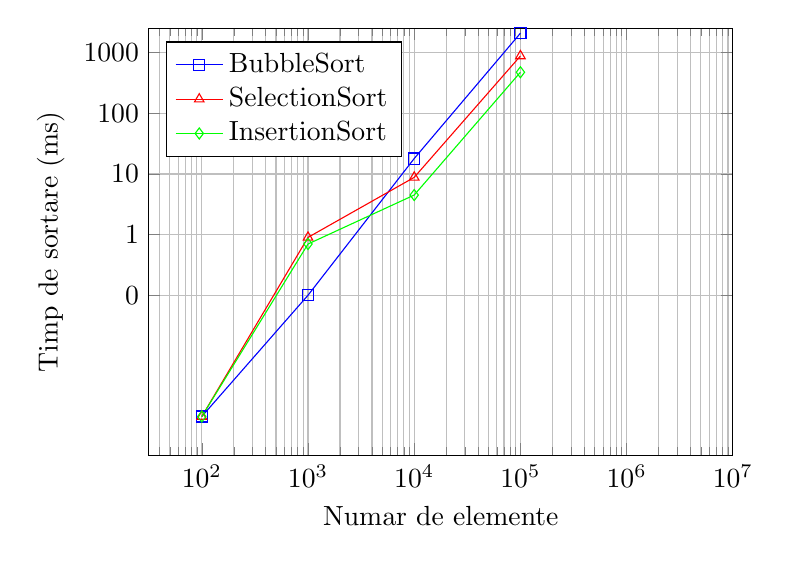
\begin{tikzpicture}
\begin{axis}[
height=7cm, width=9cm,
xlabel={Numar de elemente},
ylabel={Timp de sortare (ms)},
xmin=0, xmax=10000000,
ymin=0, ymax=25000,
xmode=log,
log basis x={10},
ymode=log,
log basis y={10},
grid=both,
legend pos=north west,
ytick={0,1,10,100,1000,10000},
yticklabels={0,1,10,100,1000,10000},
legend cell align={left},
]

\addplot[
color=blue,
mark=square,
]
coordinates {
(100,0.01)(1000,1)(10000,180)(100000,21010)
};
\addlegendentry{BubbleSort}

\addplot[
color=red,
mark=triangle,
]
coordinates {
(100,0.01)(1000,9)(10000,88)(100000,8849)
};
\addlegendentry{SelectionSort}

\addplot[
color=green,
mark=diamond,
]
coordinates {
(100,0.01)(1000,7)(10000,45)(100000,4770)
};
\addlegendentry{InsertionSort}
\end{axis}
\label{graf1}
\end{tikzpicture}
\caption{Timpul de sortare pentru BubbleSort, SelectionSort și InsertionSort reprezentat grafic}
\end{figure}
\begin{figure}
 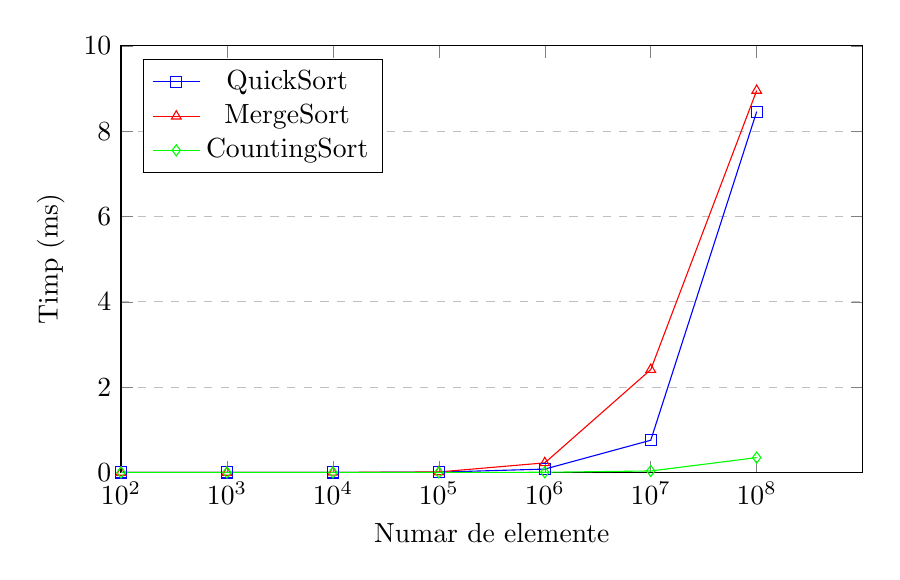
\begin{tikzpicture}
\begin{axis}[  height=7cm,   xlabel={Numar de elemente},    ylabel={Timp (ms)},    xmin=1, xmax=8,    ymin=0, ymax=10,    xtick={1,2,3,4,5,6,7,8},    xticklabels={10$^2$,10$^3$,10$^4$,10$^5$,10$^6$,10$^7$,10$^8$},    legend pos=north west,    ymajorgrids=true,    grid style=dashed,]

\addplot[    color=blue,    mark=square,    ]
    coordinates {
    (1,0.0001)(2,0.0001)(3,0.001)(4,0.007)(5,0.079)(6,0.755)(7,8.458)
    };
    
\addplot[    color=red,    mark=triangle,    ]
    coordinates {
    (1,0.0001)(2,0.0001)(3,0.001)(4,0.012)(5,0.225)(6,2.411)(7,8.952)
    };
    
\addplot[    color=green,    mark=diamond,    ]
    coordinates {
    (1,0.0001)(2,0.0001)(3,0.001)(4,0.002)(5,0.004)(6,0.035)(7,0.348)
    };

\legend{QuickSort, MergeSort, CountingSort}

\end{axis}
\label{graf2}
\end{tikzpicture}
\caption{Timpul de sortare pentru QuickSort, MergeSort și CountingSort reprezentat grafic }
\end{figure}
\begin{figure}
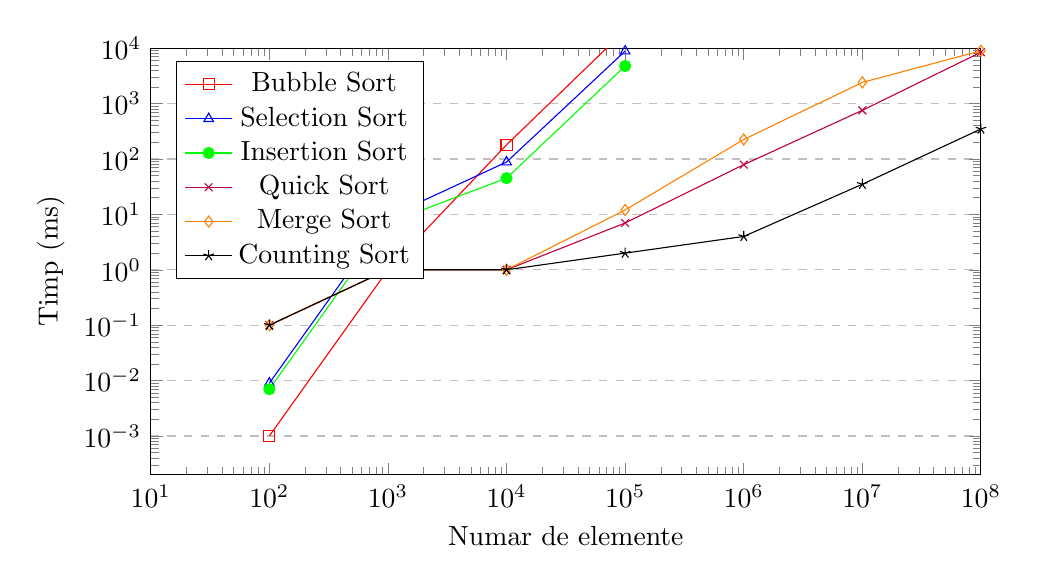
\begin{tikzpicture}
\begin{axis}[    width=\linewidth,    height=7cm,    xlabel={Numar de elemente},    ylabel={Timp (ms)},    xmin=10^1, xmax=10^8,    ymin=0, ymax=10000,    xmode=log, log basis x=10 ,    ymode=log,    legend pos=north west,    ymajorgrids=true,    grid style=dashed,]

% Bubble Sort
\addplot[    color=red,    mark=square,    ]
    coordinates {
        (100,0.001) (1000,1) (10000,180) (100000,21010) (1000000,inf)
    };
\addlegendentry{Bubble Sort}

% Selection Sort
\addplot[    color=blue,    mark=triangle,    ]
    coordinates {
        (100,0.009) (1000,9) (10000,88) (100000,8849) (1000000,inf)
    };
\addlegendentry{Selection Sort}

% Insertion Sort
\addplot[    color=green,    mark=*,    ]
    coordinates {
        (100,0.007) (1000,7) (10000,45) (100000,4770) (1000000,inf)
    };
\addlegendentry{Insertion Sort}

% Quick Sort
\addplot[    color=purple,    mark=x,    ]
    coordinates {
        (100,0.1) (1000,1) (10000,1) (100000,7) (1000000,79) (10000000,755) (100000000,8458)
    };
\addlegendentry{Quick Sort}

% Merge Sort
\addplot[    color=orange,    mark=diamond,    ]
    coordinates {
        (100,0.1) (1000,1) (10000,1) (100000,12) (1000000,225) (10000000,2411) (100000000,8952)
    };
\addlegendentry{Merge Sort}

% Counting Sort
\addplot[    color=black,    mark=star,    ]
    coordinates {
        (100,0.1) (1000,1) (10000,1) (100000,2) (1000000,4) (10000000,35) (100000000,348)
    };
\addlegendentry{Counting Sort}
\end{axis}
\label{graf3}
\end{tikzpicture}
\caption{Comparație grafică între toate metodele prezentate}
\end{figure}
Datele obținute prin repetarea experimentului, care a implicat implementarea diferitelor metode de sortare și generarea datelor de intrare prin intermediul funcției rand(), au furnizat informații relevante în ceea ce privește performanțele si limitările acestor algoritmi. Rezultatele obținute au confirmat faptul că BubbleSort este cea mai lentă metodă de sortare (Tabela \ref{tab1}), în timp ce QuickSort este cea mai rapidă, deși timpul său de execuție este similar cu cel al MergeSort (Tabela \ref{tab2}). În plus, s-a observat că, CountingSort este cel mai rapid în cazul în care elementul maxim a fost unul destul de mic. De asemenea, s-a constatat că, în unele cazuri, comportamentul rezultatelor a fost neașteptat, deoarece la primele rulari ale programului, timpii de sortare au fost mai ridicați, dar au scăzut în rulările ulterioare. \\Cu ajutorul celor 3 grafice putem vizualiza si compara grafic modificarea timpului de sortare, odată cu creșterea numărului de elemente.
\section{Comparaţia cu literatura}



O altă abordare este prezentată în "The Art of Computer Programming" scrisa de  Donald Knuth~\cite{donald1999art}. Una dintre principalele diferențe între cele două abordări este că Donald Knuth se concentrează pe analiza matematică și teoretică a algoritmilor de sortare, în timp ce experimentul realizat anterior se concentrează pe performanța practică a acestora. Un avantaj al abordării lui Knuth este acela că in cărțile sale se oferă o prezentare completă a practicilor pentru programarea eficientă. Un avantaj al experimentului descris este că a oferit o evaluare empirică a performanțelor diferitelor algoritmi de sortare utilizând date concrete de intrare. Un dezavantaj al abordării lui Knuth este că teoria poate fi complexă și greu de înțeles, pe când, experimentând cu date concrete și prezentând ideile de baza, se poate înțelege mai eficient. Un dezavantaj al experimentului descris este acela că nu au fost folosite toate datele de intrare posibile si au fost omise scenarii.  În ambele lucrări, se subliniază faptul că BubbleSort este cea mai lentă metodă de sortare, în timp ce QuickSort este cea mai rapidă și eficientă metodă, deși timpul său de execuție poate fi similar cu cel al altor metode, cum ar fi MergeSort. În plus, CountingSort este cel mai rapid atunci când elementul maxim este unul destul de mic.




\section{Concluzii şi direcţii viitoare}
Concluziile principale ale comparării algoritmilor de sortare sunt următoarele:
\begin{itemize}
    \item Viteza algoritmilor de sortare depinde de câțiva factori, cum ar fi cât de multe date trebuie sortate și cum este implementat algoritmul.
    \item  Dacă avem mai multe date de sortat, atunci vom avea nevoie de un algoritm care să poată face acest lucru rapid și eficient.

\item  Se poate îmbunătăți performanța fiecărui algoritm de sortare prin optimizare. Asta înseamnă că putem să găsim căi mai rapide sau mai eficiente pentru a-l implementa și astfel să facem ca algoritmul să sorteze datele mai repede.
\end{itemize}
În viitor, direcțiile de cercetare referitoare la compararea algoritmilor de sortare ar putea include:
\begin{itemize}
    \item Dezvoltarea și îmbunătațirea algoritmilor deja existenți
    \item Dezvoltarea tehnologiilor de memorie și procesare poate duc la optimizări ale algoritmilor de sortare existenți sau la apariția unor noi metode de sortare.
\end{itemize}
Compararea între metodele de sortare este un subiect important în informatică și programare, deoarece performanța acestor algoritmi poate avea un impact semnificativ asupra vitezei și eficienței programelor. În esență, când trebuie să sortăm un număr mare de date, trebuie să alegem cel mai bun algoritm pentru a face acest lucru cât mai rapid și mai eficient posibil.

\pagebreak
\bibliographystyle{plain}
\bibliography{bibliografie.bib}

\end{document}
